%-------------------------------------------------------------------------------
%	PACKAGES AND OTHER DOCUMENT CONFIGURATIONS
%-------------------------------------------------------------------------------


\documentclass[a4paper,12pt]{article}
\usepackage[english]{babel}
% \usepackage[latin1]{inputenc}
\usepackage{amsmath}
\usepackage{amssymb}
\usepackage{amsfonts}
\usepackage{graphicx}
\usepackage{dcolumn}
\usepackage[colorinlistoftodos]{todonotes}
\usepackage[toc,page]{appendix}
\usepackage{setspace}
% \doublespacing
\usepackage{tcolorbox}
\tcbuselibrary{skins}
\usepackage{booktabs}
\usepackage{hyperref}
\usepackage{geometry}
\usepackage[bottom]{footmisc}
\usepackage{listings}
\usepackage{longtable}
% \usepackage[demo]{graphicx}
\usepackage{subfig}
\usepackage{multirow}
\usepackage{tikz}
\usetikzlibrary{fit}
\usetikzlibrary{arrows}
\renewcommand{\arraystretch}{0.7}
\renewcommand{\labelitemi}{$\triangleright$}
 \geometry{
 a4paper,
 total={170mm,257mm},
 left=25mm,
 top=30mm,
 right=25mm,
 bottom=25mm,
 }
 \usepackage{hyperref}
 \hypersetup{
    bookmarks=true,         % show bookmarks bar?
    unicode=false,          % non-Latin characters in Acrobat’s bookmarks
    pdftoolbar=true,        % show Acrobat’s toolbar?
    pdfmenubar=true,        % show Acrobat’s menu?
    pdffitwindow=false,     % window fit to page when opened
    pdfstartview={FitH},    % fits the width of the page to the window
    pdftitle={Design_Report},    % title
    pdfauthor={Jacob Pichelman, Luca Poll},     % author
    pdfsubject={Subject},   % subject of the document
    pdfcreator={Creator},   % creator of the document
    pdfproducer={Producer}, % producer of the document
    pdfkeywords={keyword1, key2, key3}, % list of keywords
    pdfnewwindow=true,      % links in new PDF window
    colorlinks=false,       % false: boxed links; true: colored links
    linkcolor=red,          % color of internal links (change box color with linkbordercolor)
    citecolor=green,        % color of links to bibliography
    filecolor=magenta,      % color of file links
    urlcolor=cyan           % color of external links
}

\definecolor{Gray}{gray}{0.9}
% \setmonofont{Consolas}

\definecolor{background}{RGB}{39, 40, 34}
\definecolor{string}{RGB}{230, 219, 116}
\definecolor{comment}{RGB}{117, 113, 94}
\definecolor{normal}{RGB}{248, 248, 242}
\definecolor{identifier}{RGB}{166, 226, 46}

\lstset{
  language = R,                         % choose the language of the code
  linewidth = 14.75cm,
  numbers = left,                           % where to put the line-numbers
  stepnumber=1,                         % the step between two line-numbers.        
  numbersep=5pt,                        % how far the line-numbers are from the code
  numberstyle=\tiny\color{black}\ttfamily,
  backgroundcolor=\color{background},       % choose the background color. You must add \usepackage{color}
  showspaces=false,                     % show spaces adding particular underscores
  showstringspaces=false,               % underline spaces within strings
  showtabs=false,                       % show tabs within strings adding particular underscores
  tabsize=4,                            % sets default tabsize to 2 spaces
  captionpos=b,                         % sets the caption-position to bottom
  breaklines=true,                      % sets automatic line breaking
  breakatwhitespace=true,               % sets if automatic breaks should only happen at whitespace
  title=\lstname,                       % show the filename of files included with \lstinputlisting;
  basicstyle=\color{normal}\ttfamily,                   % sets font style for the code
  keywordstyle=\color{magenta}\ttfamily,    % sets color for keywords
  stringstyle=\color{string}\ttfamily,      % sets color for strings
  commentstyle=\color{comment}\ttfamily,    % sets color for comments
  emph={format_string, eff_ana_bf, permute, eff_ana_btr},
  emphstyle=\color{identifier}\ttfamily
}

% biblatex
\usepackage{biblatex}
\addbibresource{references.bib}
\usepackage{csquotes}


\begin{document}
\begin{titlepage}

\newcommand{\HRule}{\rule{\linewidth}{0.25mm}} % Defines a new command for the horizontal lines, change thickness here
\setlength{\topmargin}{-0.5in}
\center % Center everything on the page


\includegraphics[scale=0.75]{TSE.png}\\

%-------------------------------------------------------------------------------
%	HEADING SECTIONS
%-------------------------------------------------------------------------------
% \\[1.5cm]
\large \textsc{M2 EEE Machine Learning} 
\vspace{1.5cm}
% Name of your heading such as course name
\textsc{\large } % Minor heading such as course title

%-------------------------------------------------------------------------------
%	TITLE SECTION
%-------------------------------------------------------------------------------

\HRule \\[0.75cm]
{ \huge \bfseries Final Project}\\[0.5cm] % Title of your document
\HRule \\[1.75cm]
 
%-------------------------------------------------------------------------------
%	AUTHOR SECTION
%-------------------------------------------------------------------------------

\large\textsc{Andrew Boomer and Jacob Pichelmann} \\[1.5cm]

%-------------------------------------------------------------------------------
%	DATE SECTION
%-------------------------------------------------------------------------------

{\large \today}\\[0.5cm] % Date, change the \today to a set date if you want to be precise

\vfill % Fill the rest of the page with whitespace

\end{titlepage}

% -------------------------------------------------------------
% TABLE OF CONTENTS
\renewcommand{\contentsname}{Table of Contents}
\tableofcontents
% -------------------------------------------------------------

\newpage

\section{Introduction}
This report discusses and presents a replication of a selection of findings from \citeauthor{carrasco2016sample} as well as an empirical application of the methods. \citeauthor{carrasco2016sample} discusses in-sample prediction and out-of-sample forecasting in regressions with many exogenous predictors based on four dimension-reduction devices: principal components (PCA), ridge, Landweber Fridman (LF), and partial least squares (PLS). Each involves a regularization or tuning parameter that is selected through generalized cross validation (GCV) or Mallows Cp. Following \citeauthor{carrasco2016sample} we evaluate these estimators in a monte carlo simulation framework with 6 different data generating processes (DGPs). 

\section{Factor Models in Economics}

Factor models attempt to explain panels of data in terms of a smaller number of common factors that apply to each of the variables in the dataset. In the case of high dimensional data, factor models are a useful tool to reduce the dimensionality of the dataset, making estimation possible where the dataset would have been rank deficient before. A factor model on panel data can be represented as

\[\underbrace{X}_{(T \times N)} = \underbrace{F}_{(T \times r)} \underbrace{\Lambda^{'}}_{(r \times N)} + \underbrace{\xi}_{(T \times N)}\]

where $X$ denotes the matrix of observations, $F$ the underlying factors and $\Lambda$ the corresponding factor loadings. $\xi$ is an idiosyncratic shock. 

Additionally, through dimensionality reduction, factor models can find the most important variables that effect the outcome variables.
For factor models in general, a crucial part of the estimation procedure is determining the number of factors to use. This is the context that \citeauthor{carrasco2016sample} is set in. The parameter used to select the number of factors in a factor model is also known as the regularization parameter. \citeauthor{carrasco2016sample} run simulations to analyze each of the different dimension reduction devices. 

% Take two different data generating processes, (1) The eigenvalues of $\frac{X^{'}X}{T}$ are bounded and decline to zero gradually. (2) Popular factor model with a finite number, r, of factors. Here, the r largest eigenvalues grow with N, while the remaining are bounded. In both cases, $\frac{X^{'}X}{T}$ is ill-conditioned, which means the ratio of the largest to smallest eigenvalue diverges, and a regularization terms is needed to invert the matrix.

\section{Data Generating Process} \label{sec::dgp}

To study how accurate each estimation method is, \citeauthor{carrasco2016sample} simulate six different data generating processes, both in the large and small sample cases. In the large sample case, the size of the data set is $N = 200$ and $T = 500$. In the small sample case, the size is $N = 100$ and $T = 50$

% \[\underbrace{x_{t}}_{(N \times 1)} = \underbrace{\Lambda}_{(N \times r)} \underbrace{F_{t}}_{(r \times 1)} + \underbrace{\xi_{t}}_{(N \times 1)}\]

% \[\underbrace{y_{t}}_{(1 \times 1)} = \underbrace{\theta^{'}}_{(1 \times r)} \underbrace{F_{t}}_{(r \times 1)} + \underbrace{\nu_{t}}_{(1 \times 1)}\]

% \[\underbrace{y}_{(T \times 1)} = \underbrace{F}_{(T \times r)} \underbrace{\theta}_{(r \times 1)} + \underbrace{\nu}_{(T \times 1)}\]

% \[\underbrace{X}_{(T \times N)} = \underbrace{F}_{(T \times r)} \underbrace{\Lambda^{'}}_{(r \times N)} + \underbrace{\xi}_{(T \times N)}\]

\begin{itemize}
	\item DGP 1 (Few Factors Structure): \\
$\theta$ is the $(r \times 1)$ vector of ones, $r = 4$ and $r_{max} = r + 10$
	\item DGP 2 (Many Factors Structure): \\
$\theta$ is the $(r \times 1)$ vector of ones, $r = 50$ and $r_{max} = min(N, \frac{T}{2})$
	\item DGP 3 (Five Factors but only One Relevant): \\
$\theta = (1, 0_{1 \times 4})$, $r = 5$ and $r_{max} = min(r + 10, min(N, \frac{T}{2}))$

$F = [F_{1}, F_{2}^{'}]^{'}$ and $F \times F^{'} = \begin{bmatrix} 1 & 0 & 0 & 0 & 0 \\ 0 & 2 & 0 & 0 & 0 \\ 0 & 0 & 3 & 0 & 0 \\ 0 & 0 & 0 & 3 & 0 \\ 0 & 0 & 0 & 0 & 4\end{bmatrix}$

$y = \hat{F} \theta + \nu$ where $\hat{F}$ is generated from $X$ equation in DGP 3, and $\sigma_{\nu} = 0.1$
	\item DGP 4 ($x_{t}$ Has a Factor Structure but Unrelated to $y_{t}$):

$\theta$ is a vector of zeros with dimension $(r \times 1)$. $r = 5$, $r_{max} = r + 10$. $F \times F^{'}$ is defined as in DGP 3. \\

	\item DGP 5 (Eigenvalues Declining Slowly):

$\theta$ is an $(N \times 1)$ vector of ones. $r = N$, $r_{max} = min(N, \frac{T}{2})$.

$\Lambda = M \odot \xi$, with $\xi \sim (N \times N)$ matrix of $iidN(0, 1)$

$M \sim (N \times N) = \begin{bmatrix} 1 & 1 & \dotsb & 1 \\ \frac{1}{2} & \frac{1}{2} & \dotsb & \frac{1}{2} \\ \vdots & \vdots & \vdots & \vdots \\ \frac{1}{N} & \frac{1}{N} & \dotsb & \frac{1}{N}\end{bmatrix}$
	\item DGP 6 (Near Factor Model):

$\theta = 1$, $r = 1$, $r_{max} = r + 10$, $\Lambda^{'} = \frac{1}{\sqrt{N}}1_{r \times N}$
\end{itemize}



\section{Estimation Methods}

\subsection{Notation}

In matrix notation the model is 
\begin{align*}
y=\left(\begin{array}{c}
y_{1} \\
y_{2} \\
\vdots \\
y_{T}
\end{array}\right), X=\left(\begin{array}{c}
x_{1}^{\prime} \\
x_{2}^{\prime} \\
\vdots \\
x_{T}^{\prime}
\end{array}\right), \varepsilon=\left(\begin{array}{c}
\varepsilon_{1} \\
\varepsilon_{2} \\
\vdots \\
\varepsilon_{T}
\end{array}\right)
\end{align*}


where $y$ is a $(T \times 1)$ vector, $X$ is a $(T \times N)$ matrix of predictors and $\varepsilon$ is a $(T \times 1)$ vector. We then write 
\[S_{xx} = \frac{X^{T} X}{T} \quad \text{, } \quad S_{xy} = \frac{X^{T} y}{T} \]
and 
\[\widehat{y} = M_{T}^{\alpha} y = X \widehat{\delta}^{\alpha}\]

Moreover we denote as $\alpha$ the choice of penalty parameter which is obtained from one of the selection methods discussed in section \ref{sec::cv}.

For some of the estimators, we need to calculate the matrix of eigenvectors of X. Given that X is a non-square matrix in both the large and small sample cases, we decided to decompose X using the singular value decomposition (SVD). The SVD of X is represented as:

\[\underbrace{X}_{(T \times N)} = \underbrace{U}_{T \times T} \underbrace{\Sigma}_{T \times N} \underbrace{V}_{N \times N}\]

From this decomposition, we have that $U$ is the $T \times T$ matrix of orthonormalized eigenvectors of $\frac{X X^{T}}{T}$, sorted in descending order of each vectors' eigenvalues. $V^{T}$ is the matrix of orthonormalized eigenvectors of $\frac{X^{T} X}{T}$. Lastly, the diagonal of $\Sigma$ is the vector of the square root of the eigenvalues of $\frac{X^{T} X}{T}$.

In the of \citeauthor{carrasco2016sample}, $U = \hat{\psi}$ and $diag(\Sigma)^{2} = \lambda^{2}$.

\subsection{Estimators} \label{sec::estimators}

\citeauthor{carrasco2016sample} specify multiple different expressions for each of their four estimation methods. We implemented each formulation of the method to check for accuracy and computational efficiency. We unfortunately found that for some of the estimation methods, the results were not consistent between the different formulations. Additionally, where possible, we vectorized the matrix sums to improve computation time. Lastly, no matter the formulation, for some of the estimators, we were not able to get the regularization parameters to agree exactly with the tables in the paper by \citeauthor{carrasco2016sample}.


For each estimator we choose the expression that is the most computationally efficient and whose optimized parameters are the closest to the tables presented by \citeauthor{carrasco2016sample}. The four estimation methods in the paper we replicated are:

\subsubsection{Principal Components/Spectral Cutoff}

For this estimator, the implementation we use is:

\[\widehat{y} = M_{T}^{\alpha} y = \widehat{\Psi} \hat{\delta}_{PC}^{\alpha} = \widehat{\Psi} \left(\widehat{\Psi}^{\prime} \widehat{\Psi}\right)^{-1} \widehat{\Psi}^{\prime} y\]
\[\text{ where } \widehat{\Psi} = \left[\widehat{\psi}_{1}\left|\widehat{\psi}_{2}\right| \ldots \mid \widehat{\psi}_{k}\right]\]

As explained in the Notation section, $\hat{\Psi}$ is estimated from the singular value decomposition of $X$. The number of vectors $k$ included in $\hat{\Psi}$ is the regularization parameter that is optimized for the PC method. We decided to use this implementation as it was the most straightforward, agreed with the results from \citeauthor{carrasco2016sample}, and was fully vectorized.

\subsubsection{Ridge Estimator} \label{sec::ridge}

For the ridge estimator, the implementation we use is:

\[\widehat{y} = M_{T}^{\alpha} y = X \hat{\delta}_{Ridge}^{\alpha} = X (S_{xx} + \alpha I)^{-1} S_{xy}\]
where $I$ is the $(N \times N)$ identity matrix.

For this estimator, we were not able to get the estimated $\alpha$ parameter to agree with the simulation results from \citeauthor{carrasco2016sample}. We also tested the implementation of the ridge which involves the eigenvectors of $\frac{X X^{T}}{T}$:

\[M_{T}^{\alpha} y = \sum_{j=1}^{\min (N, T)} \frac{\hat{\lambda}_{j}^{2}}{\hat{\lambda}_{j}^{2}+\alpha}\left\langle y, \hat{\psi}_{j}\right\rangle_{T} \hat{\psi}_{j}\]

However, this implementation yielded estimation results that were further away from the \citeauthor{carrasco2016sample} values, and took longer to implement, so we used the specification involving the regularized inverse of $S_xx$.

\subsubsection{Landweber Fridman (LF) Estimator}

For the LF estimator, we implemented:

\[\widehat{y} = M_{T}^{\alpha} y = X \hat{\delta}_{LF}^{\alpha} = X \sum_{j=1}^{\min (N, T)} \frac{\left(1-\left(1-d \widehat{\lambda}_{j}^{2}\right)^{1 / \alpha}\right)}{\widehat{\lambda}_{j}^{2}}\left\langle y, \hat{\psi}_{j}\right\rangle_{T} \frac{X^{\prime} \hat{\psi}_{j}}{T}\]
Here $d$ denotes XXXX. We follow \citeauthor{carrasco2016sample} and choose $d = 0.018/max(\lambda^2)$.

With the LF estimator, the $\alpha$ values reported by \citeauthor{carrasco2016sample} were mostly indistiguishable from 0, so it was difficult to verify that we were implementing it correctly. However our values for the degrees of freedom (DOF) of the LF estimator were not exactly as reported, but there was no other implementation to try.

\subsubsection{Partial Least Squares (PLS) Estimator}

For the PLS estimator, we initially implemented the specification:

\[\widehat{y} = M_{T}^{\alpha} y = X V_{k}\left(V_{k}^{\prime} X^{\prime} X V_{k}\right)^{-1} V_{k}^{\prime} X^{\prime} y\]
\[\text{ where } V_{k}=\left(X^{\prime} y, \quad\left(X^{\prime} X\right) X^{\prime} y, \ldots,\left(X^{\prime} X\right)^{k-1} X^{\prime} y\right)\]

With this implementation, we were not able to get our parameter estimates for $k$ to agree with the results of \citeauthor{carrasco2016sample}. We looked at how PLS regressions were implemented in various programming softwares, and came across an implementation known as the SIMPLS algorithm by \citeauthor{de1993simpls}. This algorithm for solving PLS is as follows:

\begin{align}
\nonumber S = X^{T} y & \\
\nonumber \text{for } & i \in 1:k \\
\nonumber &\text{if } i = 1, [u, s, v] = svd(S) \\
\nonumber &\text{if } i > 1, [u, s, v] = svd(S - (P_{k}[:, i-1](P_{k}[:, i-1]^{T} P_{k}[:, i-1])^{-1} P_{k}[:, i-1]^{T} S)) \\
\nonumber &T_{k}[:, i - 1] = X R_{k}[:, i - 1] \\
\nonumber &P_{k}[:, i - 1] = \frac{X^{T} T_{k}[:, i - 1]}{T_{k}[:, i - 1]^{T}T_{k}[:, i - 1]} \\
\nonumber \widehat{y} = M^{\alpha}_{T} y &= X R_{k} (T^{T}_{k} T_{k})^{-1} T^{T}_{k} y
\end{align}

Utilising this algorithm both brought our estimated values of $k$ closer to those of \citeauthor{carrasco2016sample} and was computationally faster, so this is the method we used.

\section{Selection Methods} \label{sec::cv}

As outlined above the choice of regularization parameter is crucial. We hence implement selection on three criteria.

\begin{itemize}
	\item Generalized Cross Validation (GCV): \\
\[\hat{\alpha}=\arg \min _{\alpha \in A_{T}} \frac{T^{-1}\left\|y-M_{T}^{\alpha} y\right\|^{2}}{\left(1-T^{-1} \operatorname{tr}\left(M_{T}^{\alpha}\right)\right)^{2}}\]

	\item Mallow's Criterion: \\
\[\hat{\alpha}=\arg \min _{\alpha \in A_{T}} T^{-1}\left\|y-M_{T}^{\alpha} y\right\|^{2}+2 \widehat{\sigma}_{\varepsilon}^{2} T^{-1} \operatorname{tr}\left(M_{T}^{\alpha}\right)\]
where $\widehat{\sigma}_{\epsilon}^{2}$ is a consistent estimator of the variance of $\epsilon$. In practice this translates to the variance of $\epsilon$ being taken from the errors of the largest model, or from the model with all regressors in the case of PCA.

	\item Leave-one-out Cross Validation (LOO-CV): \\
\[\hat{\alpha}=\arg \min _{\alpha \in A_{T}} \frac{1}{T} \sum_{t=1}^{T}\left(\frac{y_{i}-\hat{y}_{i, \alpha}}{1-M_{T}^{\alpha}[ii]}\right)^{2}\]

\end{itemize}

Note that for PC and PLS, the trace of $M_{T}^{\alpha}$ is equal to the number of factors $k$. Additionally, the degrees of freedom (DOF) for each estimator is calculated as the trace of $M_{T}^{\alpha}$. 

\section{Simulation Results}

We run simulations of the six DGPs outlined in section \ref{sec::dgp} for a small sample $(N = 100, T = 50)$ and a large sample $(N=200, T=500)$ and apply all estimators discussed in section \ref{sec::estimators} with $alpha$/$k$ selected from either GCV or Mallow's Criterion. In the subsequent tables $r$ denotes the true number of factors in the underlying simulation. $k$ is the average estimated number of factors across simulations and equivalently $\alpha$ is the average penalty parameter across simulations.


    \begin{center} $(\mathrm{GCV}, N=200, T=500)$ \
        \begin{tabular}{cccccccc}
            \hline \hline 
            & & PC & PLS & \multicolumn{2}{c}{Ridge} & \multicolumn{2}{c}{LF} \\
            \hline 
            & $r$ & $k$ & $k$ & $\alpha$ & DOF & $\alpha$ & DOF \\
            \hline 
            DGP 1 & $4.00$ & $4.87$ & $7.43$ & $0.41$ & $10.98$ & $0.00$ & $0.02$ \\
            (s.e.) & $-$ & $(1.87)$ & $(3.81)$ & $(0.16)$ & $(0.81)$ & $(0.00)$ & $(0.01)$ \\
            DGP 2 & $50.00$ & $50.93$ & $109.38$ & $1.97$ & $93.09$ & $0.00$ & $0.09$ \\
            (s.e.) & $-$ & $(2.48)$ & $(18.26)$ & $(0.06)$ & $(0.94)$ & $(0.00)$ & $(0.00)$ \\
            DGP 3 & $5.00$ & $1.86$ & $1.16$ & $0.61$ & $11.15$ & $0.00$ & $0.01$ \\
            (s.e.) & $-$ & $(2.01)$ & $(1.04)$ & $(0.24)$ & $(0.93)$ & $(0.00)$ & $(0.00)$ \\
            DGP 4 & $5.00$ & $0.88$ & $1.26$ & $18.12$ & $3.87$ & $0.04$ & $0.02$ \\
            (s.e.) & $-$ & $(2.09)$ & $(1.58)$ & $(5.11)$ & $(1.54)$ & $(0.04)$ & $(0.02)$ \\
            DGP 5 & $200.00$ & $0.99$ & $8.30$ & $26.70$ & $12.08$ & $0.03$ & $0.07$ \\
            (s.e.) & $-$ & $(2.42)$ & $(9.40)$ & $(7.17)$ & $(6.81)$ & $(0.04)$ & $(0.07)$ \\
            DGP 6 & $1.00$ & $6.54$ & $1.01$ & $2.36$ & $5.28$ & $0.00$ & $0.40$ \\
            (s.e.) & $-$ & $(3.28)$ & $(0.13)$ & $(4.44)$ & $(2.04)$ & $(0.00)$ & $(0.00)$ \\
            \hline
        \end{tabular}
    \end{center}
    

In general, we obtain similar results as \citeauthor{carrasco2016sample} for PC and PLS even though our methodology for the latter departs slightly from their paper. For Ridge and LF the results are mixed. We tried all of the authors expressions for Ridge and while the implemented one (see section \ref{sec::ridge}) yields sensible results they do not match with the values the authors report. Similarly when judging the LF estimator on the degrees of freedoms used we also fail at replicating the results exactly. Given that we directly translated the authors formulas into code we are unsure where this error arises from. We take the performance of PC and PLS as indication that both the DGPs and the regularization choice were implemented correctly. 

Generally our findings are in line with \citeauthor{carrasco2016sample}. We see that PC with GCV correctly estimates the number of factors  in both cases where the number of factors is either large or small (DGP 1 and DGP 2). The performance is better in the large sample. Contrarily Mallows' Criterion tends to overestimate the number of factors when the true number of factors is small (DGP 1, DGP 3, DGP 4 and DGP 6). When the number of factors is small but only one factor is a relevant predictor of $y_t$ (DGP 3) GCV slightly overestimates the number of relevant factors. Here again Mallows' Criterion performs worse and heavily overestimates the number of relevant factors. When eigenvalues decline gradually (DGP 5) GCV yields a small number of relevant factors both in the large sample and in the small sample case. Mallow again estimates a greater number of factors. Lastly, in DGP 6, where the eigenvalues are small in magnitude, both GCV and Mallows Criterion overestimate the number of relevant factors. 


    \begin{center} $(\mathrm{GCV}, N=100, T=50)$ \
        \begin{tabular}{cccccccc}
            \hline \hline 
            & & PC & PLS & \multicolumn{2}{c}{Ridge} & \multicolumn{2}{c}{LF} \\
            \hline 
            & $r$ & $k$ & $k$ & $\alpha$ & DOF & $\alpha$ & DOF \\
            \hline 
            DGP 1 & $4.00$ & $4.78$ & $4.23$ & $1.25$ & $7.83$ & $0.00$ & $0.15$ \\
            (s.e.) & $-$ & $(2.08)$ & $(3.43)$ & $(0.56)$ & $(1.23)$ & $(0.00)$ & $(0.02)$ \\
            DGP 2 & $50.00$ & $19.50$ & $3.31$ & $0.99$ & $23.37$ & $0.00$ & $0.51$ \\
            (s.e.) & $-$ & $(6.06)$ & $(5.23)$ & $(0.02)$ & $(0.14)$ & $(0.00)$ & $(0.07)$ \\
            DGP 3 & $5.00$ & $1.99$ & $1.16$ & $1.02$ & $9.33$ & $0.00$ & $0.10$ \\
            (s.e.) & $-$ & $(2.33)$ & $(1.07)$ & $(0.39)$ & $(1.02)$ & $(0.00)$ & $(0.01)$ \\
            DGP 4 & $5.00$ & $1.18$ & $1.34$ & $8.70$ & $5.00$ & $0.02$ & $0.21$ \\
            (s.e.) & $-$ & $(2.61)$ & $(1.70)$ & $(2.95)$ & $(1.73)$ & $(0.02)$ & $(0.21)$ \\
            DGP 5 & $100.00$ & $1.34$ & $3.73$ & $12.47$ & $3.99$ & $0.01$ & $0.41$ \\
            (s.e.) & $-$ & $(3.28)$ & $(4.14)$ & $(4.70)$ & $(2.96)$ & $(0.02)$ & $(0.38)$ \\
            DGP 6 & $1.00$ & $3.32$ & $1.17$ & $5.85$ & $2.59$ & $0.10$ & $0.13$ \\
            (s.e.) & $-$ & $(3.15)$ & $(0.91)$ & $(3.99)$ & $(1.95)$ & $(0.08)$ & $(0.25)$ \\
            \hline
        \end{tabular}
    \end{center}
    

    \begin{center} $(\mathrm{Mallow}, N=100, T=50)$ \
        \begin{tabular}{cccccccc}
            \hline \hline 
            & & PC & PLS & \multicolumn{2}{c}{Ridge} & \multicolumn{2}{c}{LF} \\
            \hline 
            & $r$ & $k$ & $k$ & $\alpha$ & DOF & $\alpha$ & DOF \\
            \hline 
            DGP 1 & $4.00$ & $14.00$ & $14.00$ & $0.00$ & $14.00$ & $0.00$ & $0.78$ \\
            (s.e.) & $-$ & $(0.00)$ & $(0.00)$ & $(0.00)$ & $(0.00)$ & $(0.00)$ & $(0.03)$ \\
            DGP 2 & $50.00$ & $25.00$ & $25.00$ & $0.00$ & $25.00$ & $0.00$ & $0.66$ \\
            (s.e.) & $-$ & $(0.00)$ & $(0.00)$ & $(0.00)$ & $(0.00)$ & $(0.00)$ & $(0.01)$ \\
            DGP 3 & $5.00$ & $15.00$ & $15.00$ & $0.00$ & $15.00$ & $0.00$ & $0.51$ \\
            (s.e.) & $-$ & $(0.00)$ & $(0.00)$ & $(0.00)$ & $(0.00)$ & $(0.00)$ & $(0.04)$ \\
            DGP 4 & $5.00$ & $15.00$ & $15.00$ & $0.00$ & $15.00$ & $0.00$ & $0.51$ \\
            (s.e.) & $-$ & $(0.00)$ & $(0.00)$ & $(0.00)$ & $(0.00)$ & $(0.00)$ & $(0.04)$ \\
            DGP 5 & $100.00$ & $25.00$ & $25.00$ & $0.00$ & $25.00$ & $0.00$ & $0.87$ \\
            (s.e.) & $-$ & $(0.00)$ & $(0.00)$ & $(0.00)$ & $(0.00)$ & $(0.00)$ & $(0.04)$ \\
            DGP 6 & $1.00$ & $11.00$ & $11.00$ & $0.00$ & $11.00$ & $0.00$ & $1.00$ \\
            (s.e.) & $-$ & $(0.00)$ & $(0.00)$ & $(0.00)$ & $(0.00)$ & $(0.00)$ & $(0.00)$ \\
            \hline
        \end{tabular}
    \end{center}
    

Moving to the predictive power of our estimators we plot the in-sample MSE for all cases discussed above.\footnote{Due to computational limitations we limit the number of simulations for the large sample to 25.} This setting also allows to evaluate the performance of Ridge and LF. We can see that LF consistently performs worst in terms of in-sample MSE and that this behaviour is especially pronounced for DGP 1, DGP 2 and DGP 3. Contrarily, PLS yields a comparably small in-sample MSE across all DGPs and performs especially well when eigenvalues are small in magnitude. Ridge and PC perform similarly across all DGPs. 

\begin{table}[h! ]
     \centering
     \caption*{N = 100, T=50, Simulations = 1000}
     \begin{tabular}{c c}
     DGP 1 & DGP 2 \\
         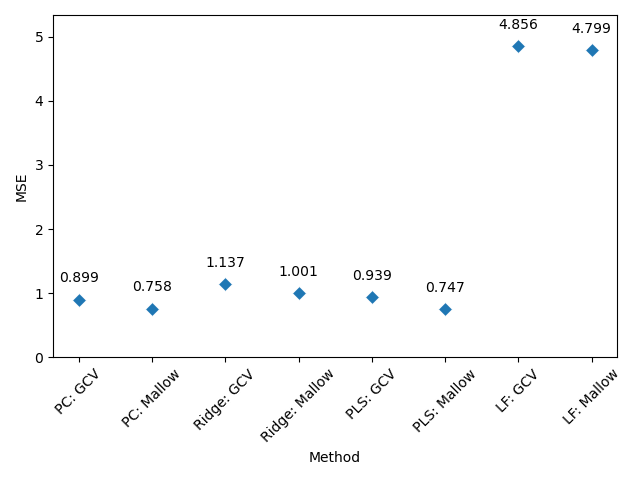
\includegraphics[width=0.45\textwidth]{figures/N100_T50_DGP1_Sims1000.png} & 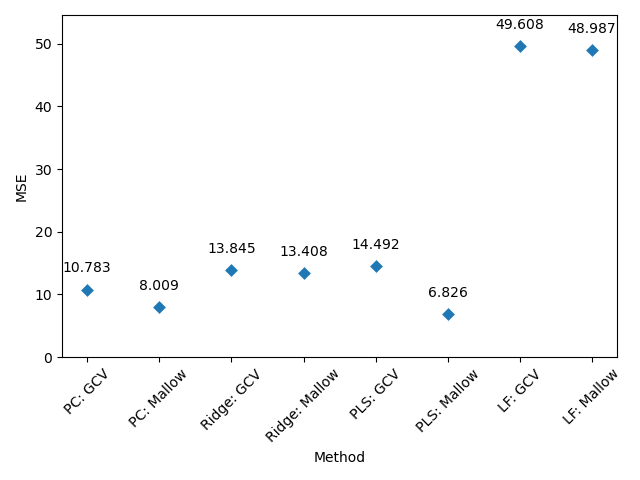
\includegraphics[width=0.45\textwidth]{figures/N100_T50_DGP2_Sims1000.png} \\
                 DGP 3 & DGP 4 \\
         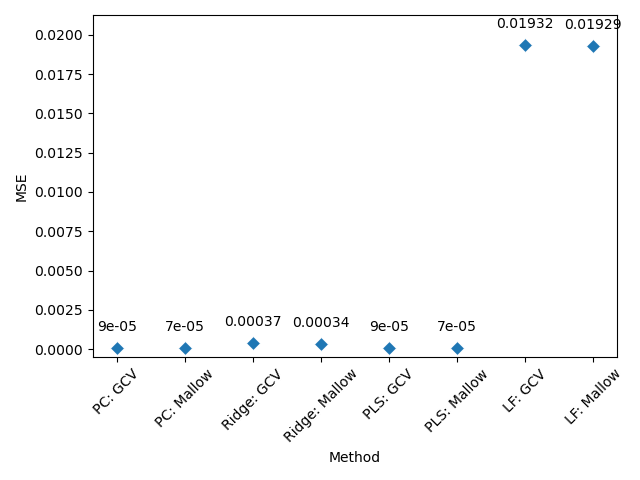
\includegraphics[width=0.45\textwidth]{figures/N100_T50_DGP3_Sims1000} &
         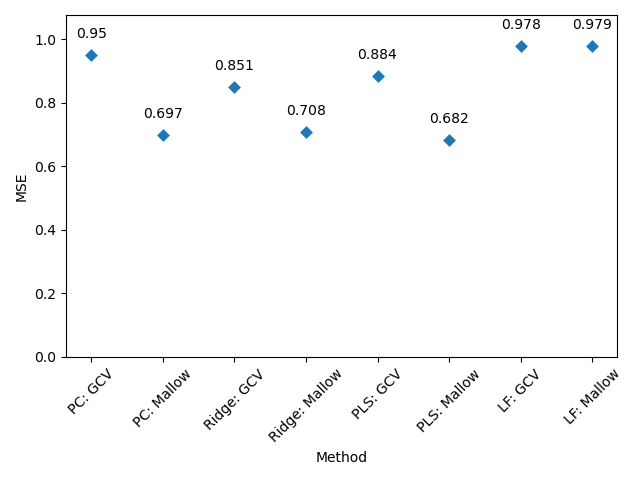
\includegraphics[width=0.45\textwidth]{figures/N100_T50_DGP4_Sims1000} \\
         DGP 5 & DGP 6 \\
         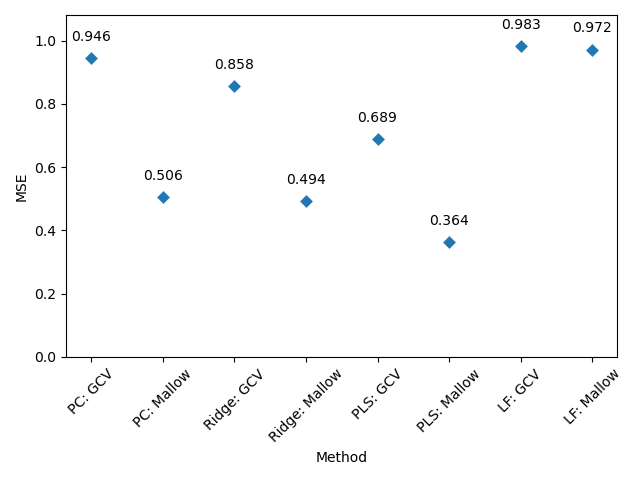
\includegraphics[width=0.45\textwidth]{figures/N100_T50_DGP5_Sims1000} &
         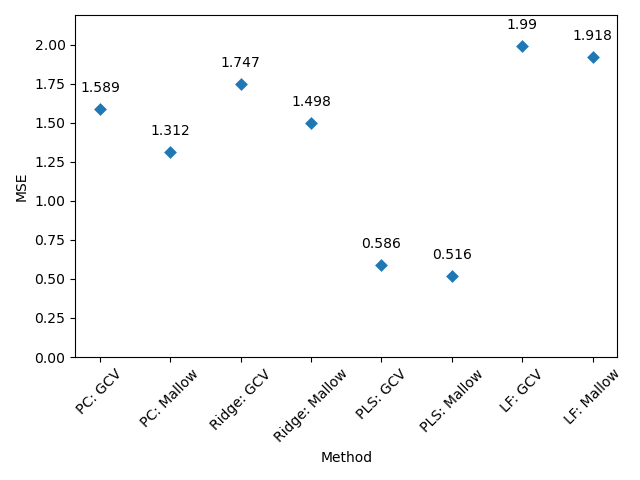
\includegraphics[width=0.45\textwidth]{figures/N100_T50_DGP6_Sims1000}
     \end{tabular}
\end{table}

\begin{table}[h! ]
    \centering
    \caption*{N = 200, T=500, Simulations = 25}
    \begin{tabular}{c c}
    DGP 1 & DGP 2 \\
        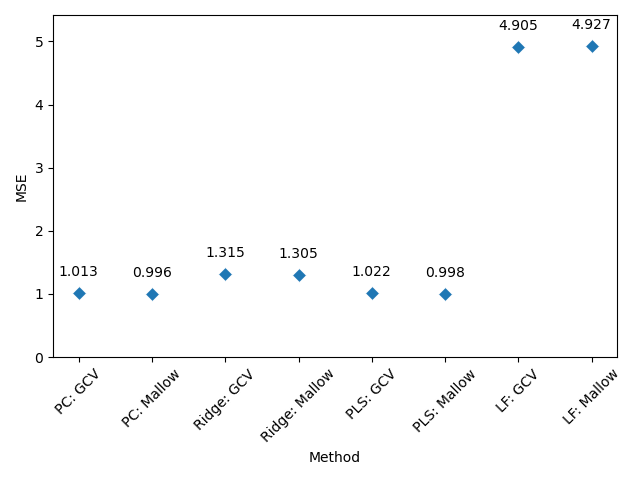
\includegraphics[width=0.45\textwidth]{figures/N200_T500_DGP1_Sims25.png} & 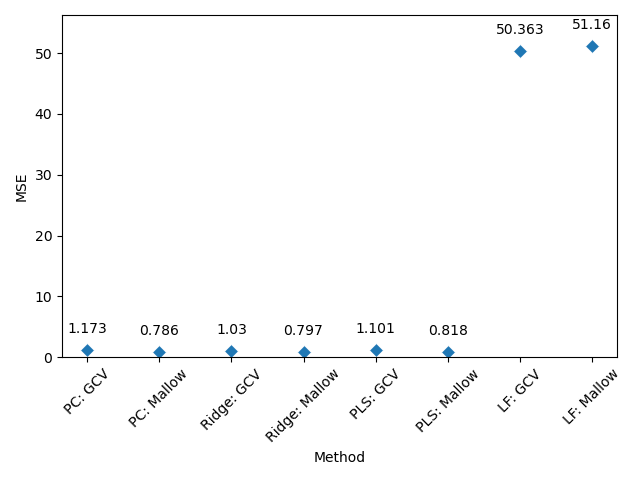
\includegraphics[width=0.45\textwidth]{figures/N200_T500_DGP2_Sims25.png} \\
        DGP 3 & DGP 4 \\
        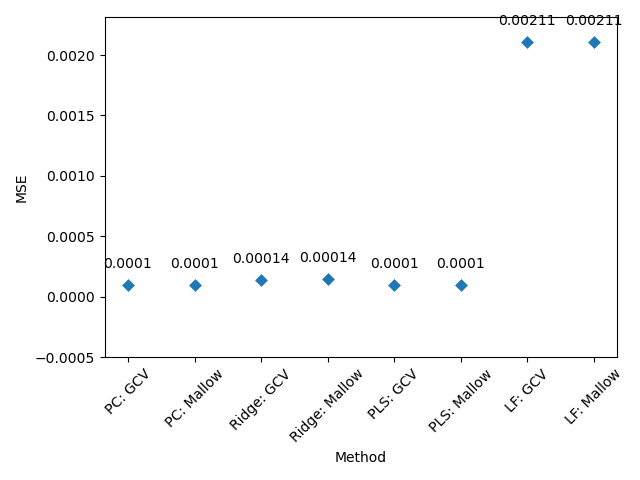
\includegraphics[width=0.45\textwidth]{figures/N200_T500_DGP3_Sims25} &
        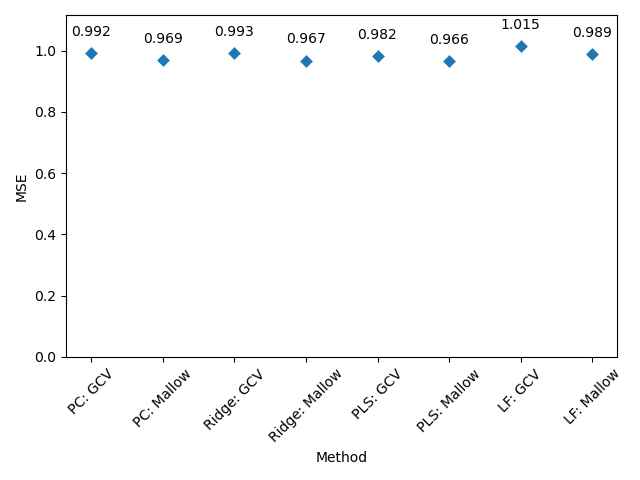
\includegraphics[width=0.45\textwidth]{figures/N200_T500_DGP4_Sims25} \\
        DGP 5 & DGP 6 \\
        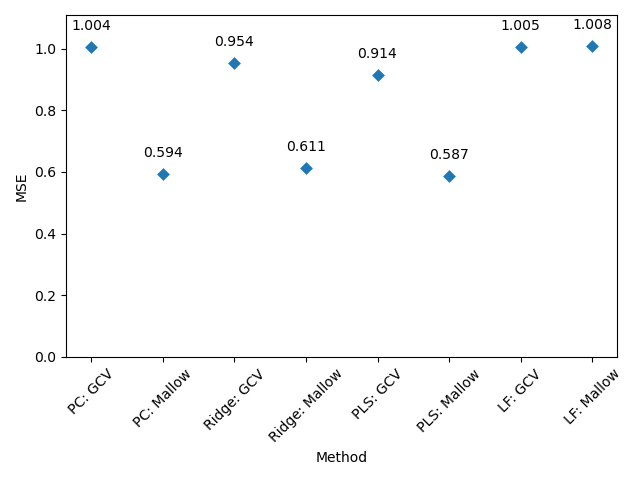
\includegraphics[width=0.45\textwidth]{figures/N200_T500_DGP5_Sims25} &
        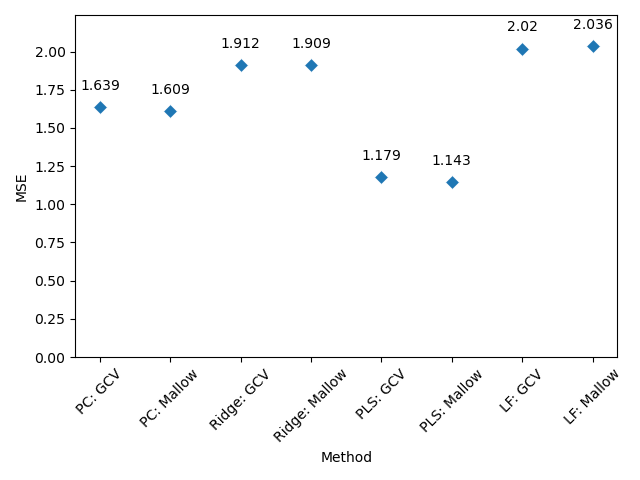
\includegraphics[width=0.45\textwidth]{figures/N200_T500_DGP6_Sims25}
    \end{tabular}
\end{table}

From these simulations we can derive key insights for the subsequent empirical application. 
\begin{itemize}
	\item If the underlying factor structure is few factors we expect PC with GCV to yield good estimates of the true number of factors. 
	\item We expect to over-estimate the number of factors when using Mallows' Criterion.
	\item In terms of forecasting performance the simulations indicate that PLS consistently returns the smallest in-sample MSE whereas LF performs worst.
	\item We do not expect to see pronounced differences in forecasting performance between PC and Ridge. 
\end{itemize}

\section{Empirical Application}
\subsection{Introduction and Data}
Building on the long history of machine learning in forecasting macroeconomic variables\footnote{See e.g. \cite{swanson1997model}, \cite{stock1998comparison} or \cite{stock2002macroeconomic}.} we use the Federal Reserve Bank's monthly database (FRED-MD) to apply the estimators discussed above on real data.\footnote{Unfortunately we were unable to use (1) \cite{gu2020empirical} as TSE does not have access to WDRS returns, (2) \cite{ludvigson2009macro} as only data on the resulting factors is available or (3) \cite{stock2002macroeconomic} as they do not offer any replication data.} This database was established for empirical analysis that requires 'big data' and hence constitutes an ideal environment to employ the methods discussed above. We took inspiration from the work of \citeauthor{coulombe2020machine} but limit ourselves to PC, Ridge, PLS and LF. 
The dataset contains 134 monthly US macroeconomic and financial indicators observed from January 1959 to January 2021. An overview of all variables is given in the appendix. 
Following \citeauthor{coulombe2020machine} we predict three indicators which are of key economic interest, namely Industrial Production (INDPRO), Unemployment Rate (UNRATE), and housing starts (HOUST).\footnote{Fortunately \cite{mccracken2016fred}, the accompanying paper of the dataset, outlines a transformation method for each variable to achieve stationarity. We apply those transformations in our data preparation.}
For each of these variables of interest $Y_t$ we follow \citeauthor{coulombe2020machine} in defining the forecast objective as

\begin{align*}
	y_{t+h} = (1/h) ln(Y_{t+h}/Y_t)
\end{align*}

where $h$ denotes the number of periods ahead.  Given that $Y_t$ has been transformed to be $I(1)$\footnote{See \cite{mccracken2016fred} for details.}, this translates to forecasting the average growth rate over the period $[t + 1, t + h]$ \parencite{stock2002macroeconomic}. This allows us to assess the performance of our predictive methods for further periods ahead.
Given the nature of the data we expect the underlying factor structure to be similar to DGP 1, i.e. few factors. \parencite{mccracken2016fred} If this assumption holds true we expect PC with GCV to correctly estimate the number of factors. 

\subsection{Evaluation}
We evaluate the performance of our methods on the out of sample MSE. To be able to compute this metric we split our data into a training and a test set where the former spans all observations from January 1959 to May 2008 amounting to 80\% of the data.\footnote{We found the results to be robust for training sizes between 0.6 and 0.9 (not reported), hence we see the cutoff amid the great recession as not problematic.} Denoting $N$ the number of observations in the test set we calculate the out of sample MSE as
\begin{align*}
	    MSE = \frac{1}{N} \sum_{i=1}^N (Y_i - \widehat{Y}_i)^2
\end{align*}
where $\widehat{Y}_i = \widehat{\Psi} \widehat{\delta}_{pc}$ for PCA and $\widehat{Y}_i = X_{test} \widehat{\delta}_{m}, m \in \{R, LF, PLS\}$ for all other models. 

We conduct forecasts for $h = \{1, 3, 9\}$ periods ahead. Subsequently we report results similar to the simulation framework; we provide tables showing for each combination of estimator and parameter selection method the estimated penalty parameter/the number of factors as well as the degrees of freedom and the resulting out of sample MSE for $h=1$. Moreover, we visualize the out of sample MSE to ease comparison across methods and settings.

\subsection{Results and Discussion}
From tables \ref{tab::indpro} to \ref{tab::houst} we can immediately see that the estimated factor structure as well as the chosen penalty parameters are remarkably stable across both selection criteria and variables of interest. We cautiously take this as indication for the underlying macro data to indeed exhibit a stable factor structure, i.e. that economic variables are driven by a set of common underlying factors. \parencite{mccracken2016fred} The number of estimated factors ranges from 9 to 15 depending on the setting and choice of method, which is in line with the literature. \parencite{mccracken2016fred}
Moreover, we can see that Mallows' Criterion again estimates a larger number of factors than GCV, which is exactly the behaviour we expected from the simulation results. 
In terms of forecasting power, we can see that LF yields the smallest out of sample MSE for $h=1$ across all variables of interest. This is somewhat surprising given its poor performance in the simulation framework when evaluated on the in-sample MSE. \citeauthor{carrasco2016sample} note, however, that its out-of-sample forecasting power is high, which validates our findings. Still, the difference to Ridge is close to negligible. 

\begin{table}[h!]
\centering
\caption{$Y_t = INDPRO$}
\label{tab::indpro}
	\begin{tabular}{lrrr}
\toprule
       Method &  OOS MSE, $h =1$ &  $alpha$/$k$ &  DOF \\
\midrule
      LF: GCV & 0.000126 &   0.0001 & 14.532053 \\
   LF: Mallow & 0.000126 &   0.0001 & 14.532053 \\
      PC: GCV & 0.000162 &  13.0000 & 13.000000 \\
   PC: Mallow & 0.000162 &  15.0000 & 15.000000 \\
     PLS: GCV & 0.002139 &  15.0000 & 15.000000 \\
  PLS: Mallow & 0.002139 &  15.0000 & 15.000000 \\
   Ridge: GCV & 0.000130 &   0.1170 & 20.074885 \\
Ridge: Mallow & 0.000130 &   0.1170 & 20.074885 \\
\bottomrule
\end{tabular}
\end{table}

\begin{table}[h!]
\centering
\caption{$Y_t = UNRATE$}
\label{tab::unrate}
\begin{tabular}{lrrr}
\toprule
       Method &  OOS MSE, $h =1$ &  $alpha$/$k$ &  DOF \\
\midrule
      LF: GCV & 0.001488 &   0.0001 & 14.418940 \\
   LF: Mallow & 0.001488 &   0.0001 & 14.418940 \\
      PC: GCV & 0.002247 &   9.0000 &  9.000000 \\
   PC: Mallow & 0.002276 &  15.0000 & 15.000000 \\
     PLS: GCV & 0.031782 &  13.0000 & 13.000000 \\
  PLS: Mallow & 0.063822 &  15.0000 & 15.000000 \\
   Ridge: GCV & 0.001779 &   0.1170 & 20.008091 \\
Ridge: Mallow & 0.001779 &   0.1170 & 20.008091 \\
\bottomrule
\end{tabular}
\end{table}

\begin{table}[h!]
\centering
\caption{$Y_t = HOUST$}
\label{tab::houst}
\begin{tabular}{lrrr}
\toprule
       Method &  OOS MSE, $h =1$ &  $alpha$/$k$ &  DOF \\
\midrule
      LF: GCV & 0.007627 &   0.0001 & 14.441119 \\
   LF: Mallow & 0.007627 &   0.0001 & 14.441119 \\
      PC: GCV & 0.010409 &  15.0000 & 15.000000 \\
   PC: Mallow & 0.010409 &  15.0000 & 15.000000 \\
     PLS: GCV & 0.329750 &  11.0000 & 11.000000 \\
  PLS: Mallow & 0.238590 &  15.0000 & 15.000000 \\
   Ridge: GCV & 0.008906 &   0.1170 & 20.052968 \\
Ridge: Mallow & 0.008906 &   0.1170 & 20.052968 \\
\bottomrule
\end{tabular}
\end{table}

Comparing the performance across variables we make the interesting finding that the PLS performs very poorly when predicting $HOUST$. We therefore report for each time horizon also the subset of only $INDPRO$ and $UNRATE$ to increase readability. Generally PLS yields the highest out of sample MSE while Ridge and LF perform best. This pattern was not present in the evaluation of simulation results, hence investigating this further, also with respect to the empirical context, might yield interesting insights. This is, however, out of scope of this report.

In line with the findings of \citeauthor{coulombe2020machine} we observe that the performance increases for further periods ahead. This finding holds true for all estimators and all variables of interest. 


%\newcolumntype{M}[1]{>{\centering\arraybackslash}m{#1}}
\begin{table}[h!]
    \centering
    \begin{tabular}{c}
        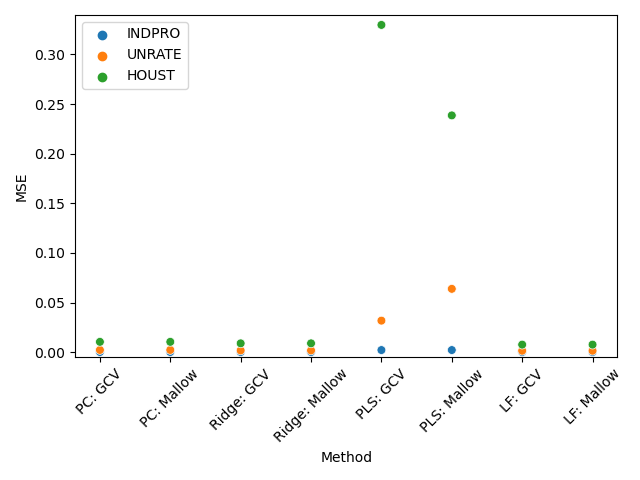
\includegraphics[width=0.6\textwidth]{figures/MSE_oos_h1.png} \\
        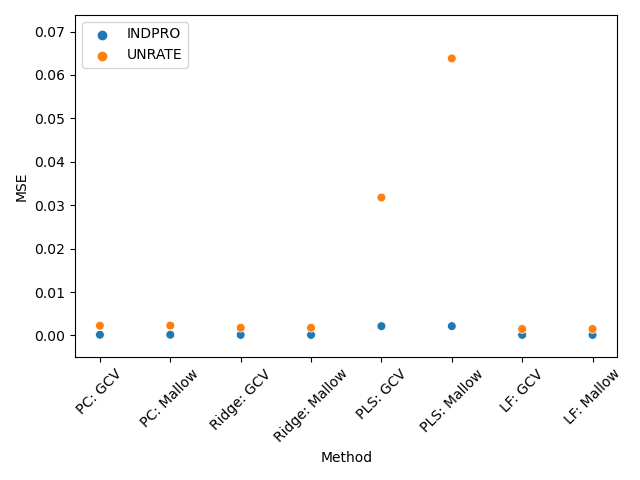
\includegraphics[width=0.6\textwidth]{figures/MSE_oos_h1_noHOUST.png}
    \end{tabular}
    \caption*{Out of sample MSE, $h = 1$}
\end{table}

\clearpage

\begin{table}[h!]
    \centering
    \begin{tabular}{c c}
        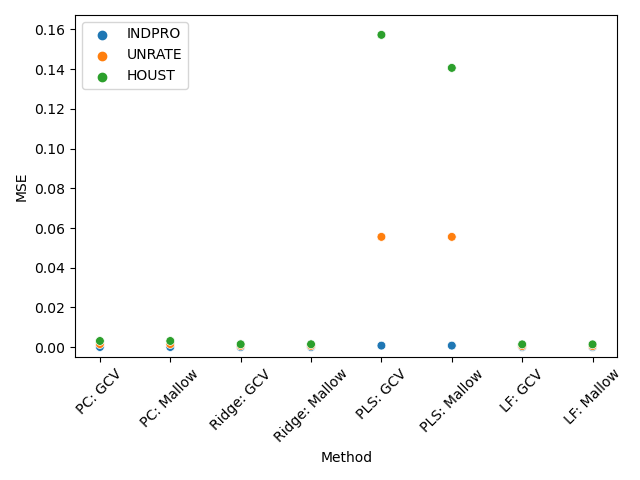
\includegraphics[width=0.4\textwidth]{figures/MSE_oos_h3.png} & 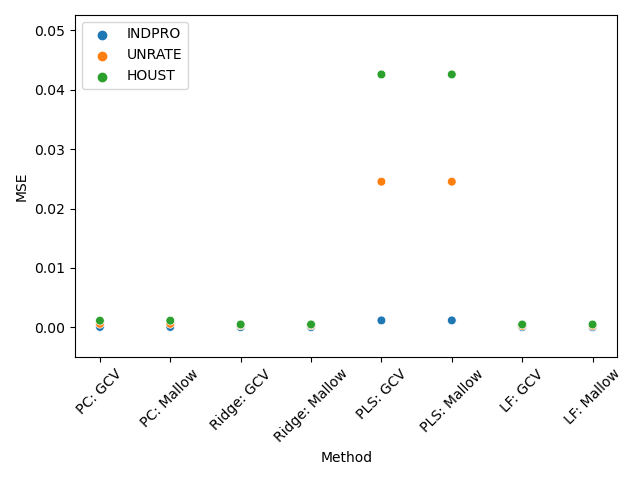
\includegraphics[width=0.4\textwidth]{figures/MSE_oos_h9.png} \\
        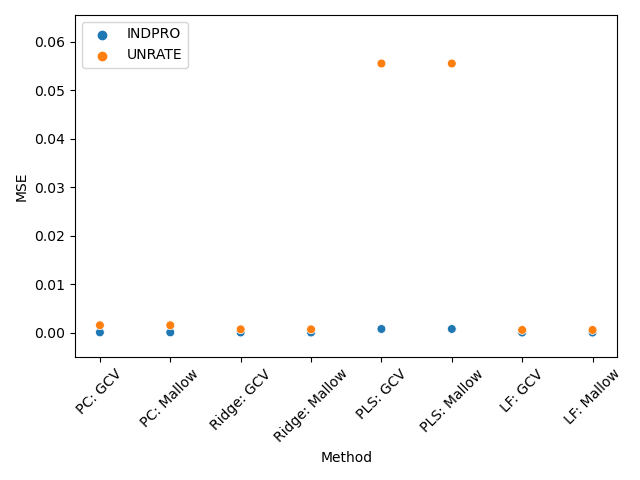
\includegraphics[width=0.4\textwidth]{figures/MSE_oos_h3_noHOUST.png} &
        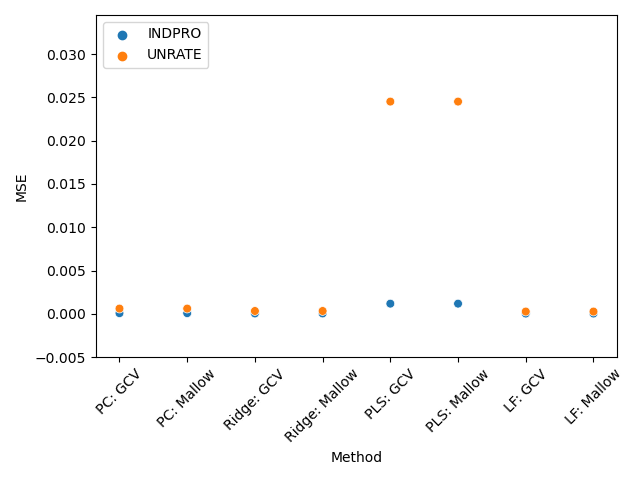
\includegraphics[width=0.4\textwidth]{figures/MSE_oos_h9_noHOUST.png} \\
        Out of sample MSE, $h = 3$ & Out of sample MSE, $h = 9$
    \end{tabular}
\end{table}

\section{Conclusion}
For this report we implemented four dimension-reduction devices (PC, PLS, Ridge and LF) and evaluated their performance in a simulation framework and on real data. From the simulation framework we found, in line with \citeauthor{carrasco2016sample}, that PC with GCV correctly estimates the number of factors when the true number of factors is small. In conjunction with the literature on macroeconomic forecasting we were able to use this insight to evaluate estimated number of factors from real world data more cautiously. In this sense, this report can provide guidance in selecting the appropriate dimension-reduction device depending on the empirical context the research question is situated in. 

\clearpage 

\nocite{*}
\printbibliography

\clearpage

\section*{Appendix}

\subsection*{Data Dictionary}
\begin{figure}[h!]
        \centering
        \caption*{Group 1: Output and income}
        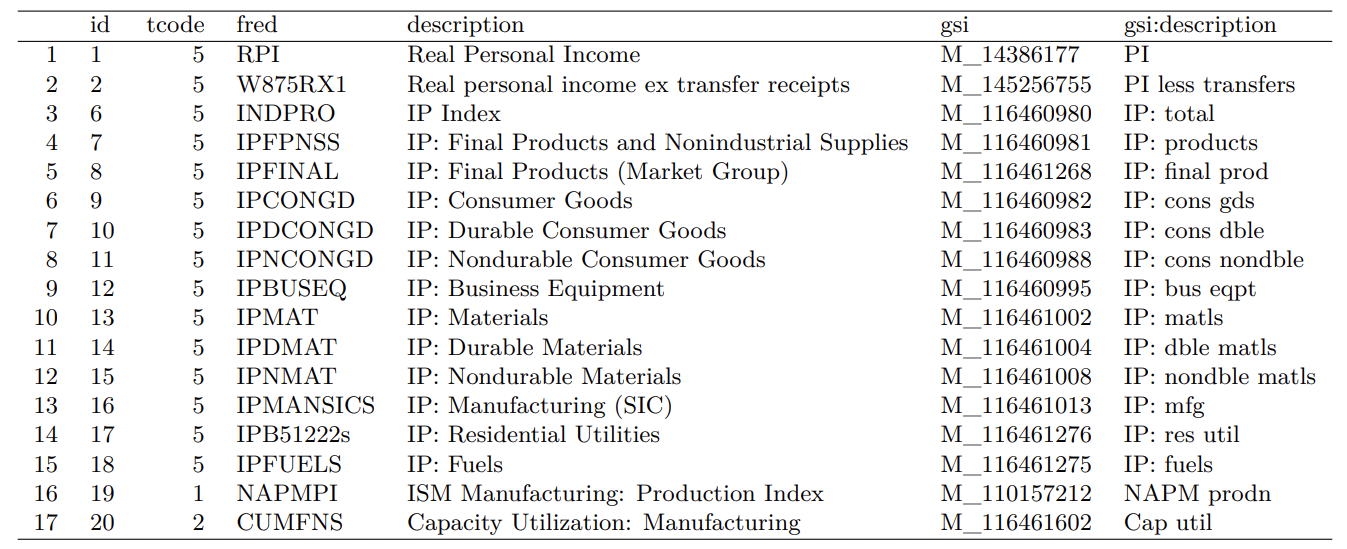
\includegraphics[width=0.9\textwidth]{figures/G1.png}
\end{figure}

\begin{figure}
        \centering
        \caption*{Group 2: Labour market}
        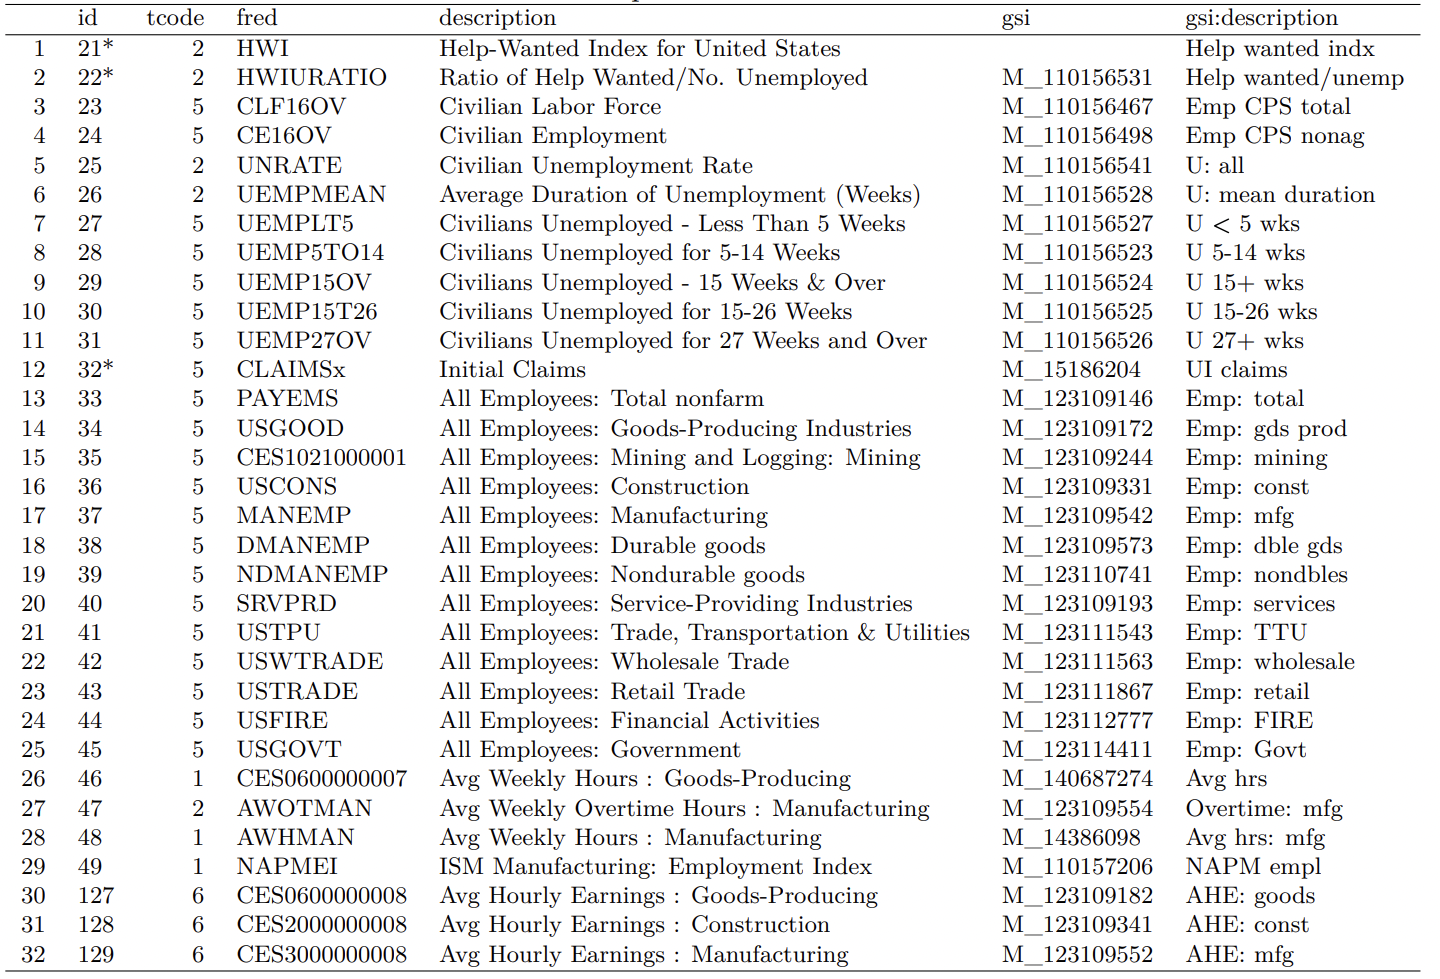
\includegraphics[width=0.9\textwidth]{figures/G2.png}
\end{figure}

\begin{figure}
        \centering
        \caption*{Group 3: Housing}
        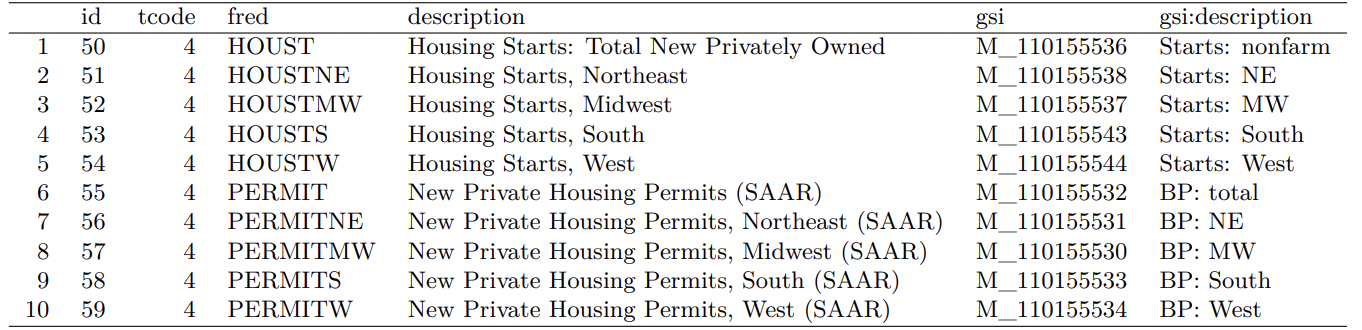
\includegraphics[width=0.9\textwidth]{figures/G3.png}
\end{figure}

\begin{figure}
        \centering
        \caption*{Group 4: Consumption, orders and inventories}
        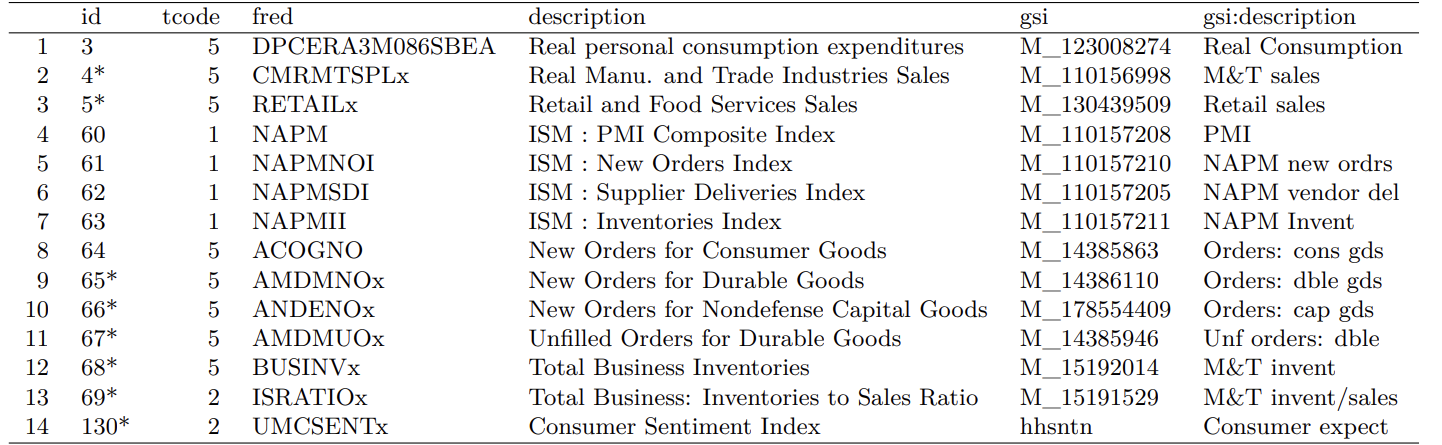
\includegraphics[width=0.9\textwidth]{figures/G4.png}
\end{figure}

\begin{figure}
        \centering
        \caption*{Group 5: Money and credit}
        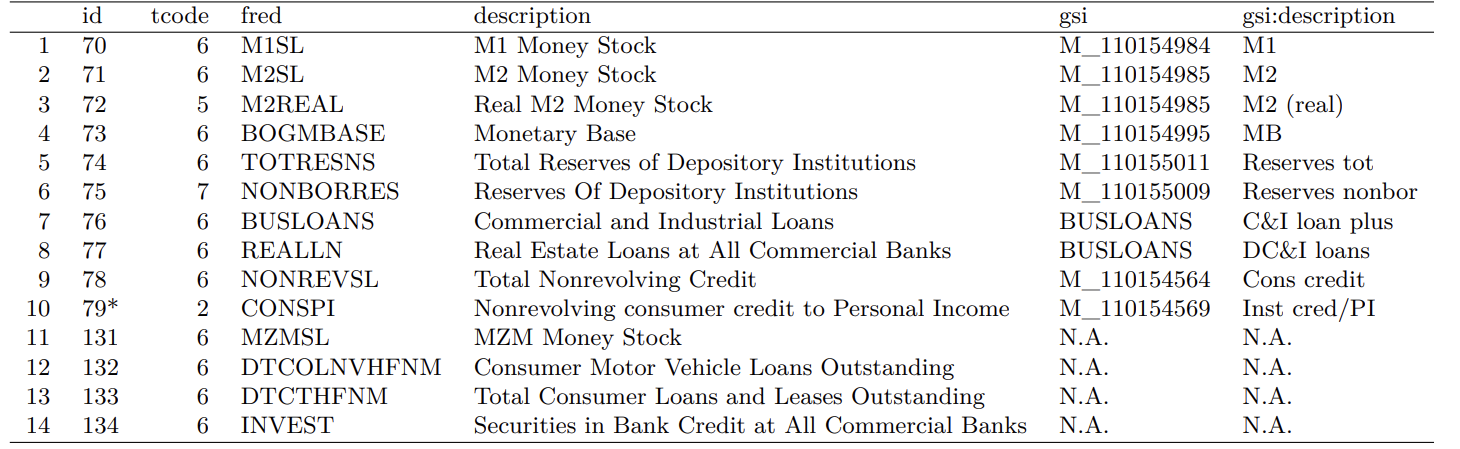
\includegraphics[width=0.9\textwidth]{figures/G5.png}
\end{figure}

\begin{figure}
        \centering
        \caption*{Group 6: Interest and exchange rates}
        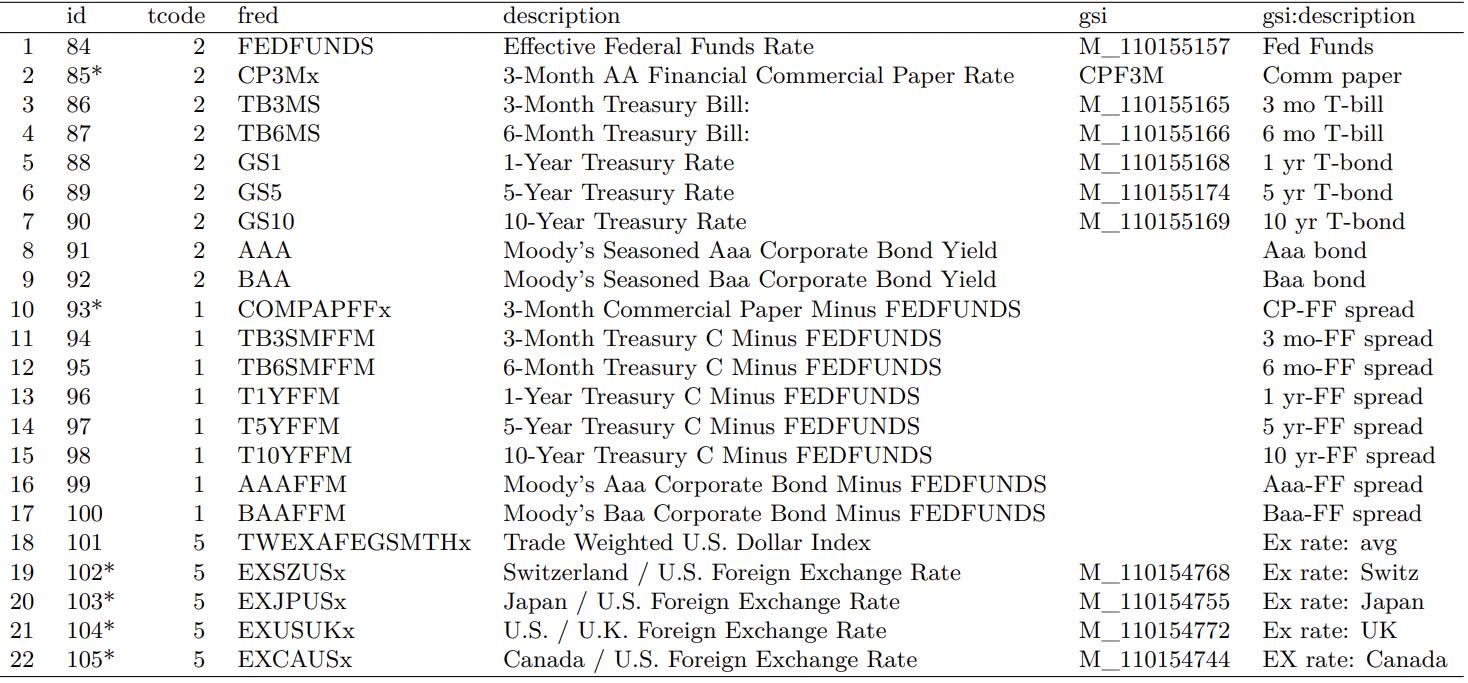
\includegraphics[width=0.9\textwidth]{figures/G6.png}
\end{figure}

\begin{figure}
        \centering
        \caption*{Group 7: Prices}
        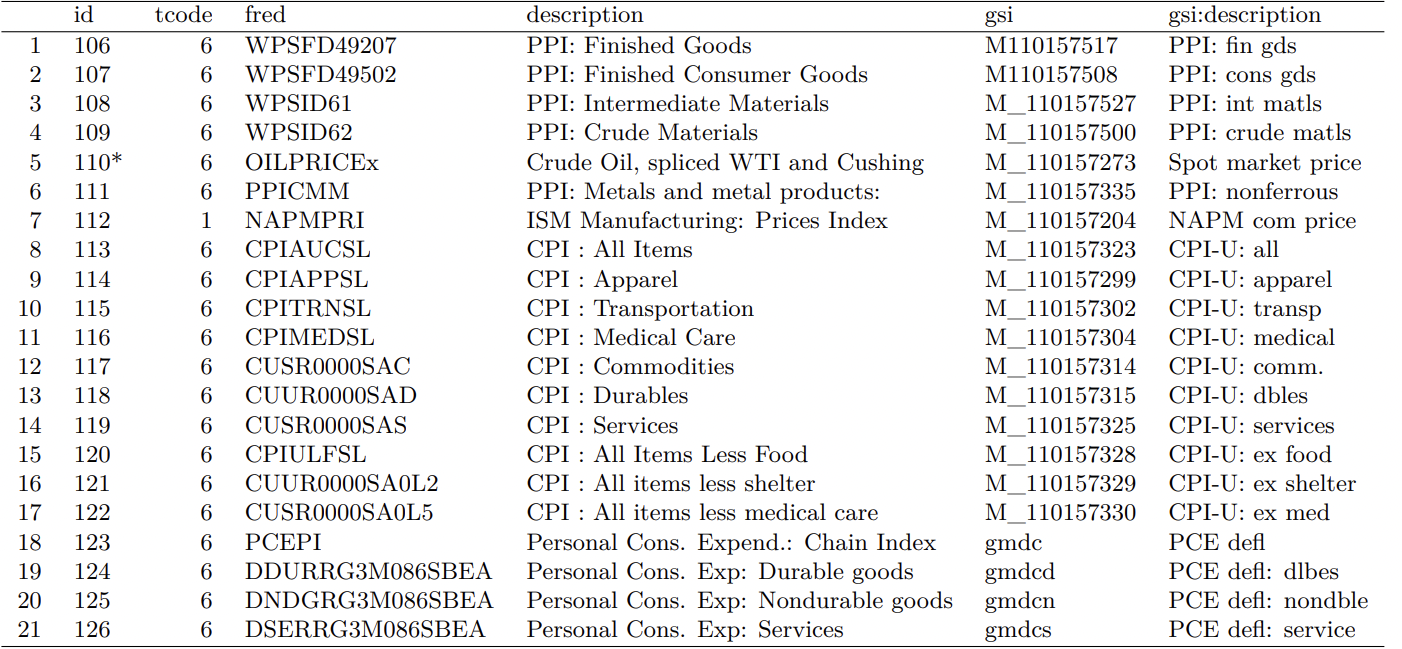
\includegraphics[width=0.9\textwidth]{figures/G7.png}
\end{figure}

\begin{figure}
        \centering
        \caption*{Group 8: Stock market}
        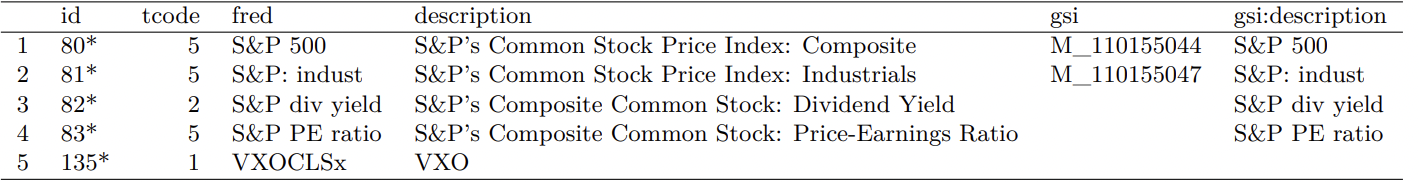
\includegraphics[width=0.9\textwidth]{figures/G8.png}
\end{figure}








\end{document}




